% % % % % % % % % % % % % % % % % % % % % % % % % % % % % % % % % % % % %
% Chapter: Introduction
% % % % % % % % % % % % % % % % % % % % % % % % % % % % % % % % % % % % %
\chapter{Introduction}
\label{chp:intro}
\pinfo{Short about Rebel}
Large systems often suffer from domain knowledge that is implicit, incomplete,
out of date or contains ambiguous definitions. This is what \textit{Rebel} aims
to solve~\cite{stoel2016solving}. The toolchain of \textit{Rebel} can be used to
check, simulate and visualize the specifications, allowing to reason about the
final product~\cite{stoel2015case}. Checking is done based on bounded model checking
by using the \textit{Z3} solver.\\
\\
\pinfo{Aim of project}
Generators are being used to generate a system from the \textit{Rebel}
specifications. The generated system provides an \textit{API} in order to work with the
specified product and handles the database connectivity. However, the
implementation of the generated system is not checked against the
specifications, meaning that the generated system is perhaps not doing what it
is supposed to do according to its specifications. The aim of this project is to
improve this, by automatically testing the generated system against a
\textit{Rebel} specification.

% % % % % % % % % % % % % % % % % % % % % % % % % % % % % % % % % % % % %
% Section: Problem statement
\section{Problem statement}
\pinfo{Translation from generator and why automatically}
From the \textit{Rebel} specifications, a system can be generated by the
generator. However, neither the generator nor the generated program is being
tested against the specification. Thus it could be that the generated system
doesn't work according to what was specified in the \textit{Rebel}
specification. Although the generator should translate everything correctly, we
cannot assume that it actually does translate it correctly for each case and
that the implementation works as expected.\\
\\
Currently, there are no tests for the generator or the generated system, during
the development of the generator the results are being checked manually. Testing
is a major cost factor in software development, with test automation being
proposed as one of the solutions to reduce these
costs~\cite{ramler2006economic}. We aim for an approach such that much of the
testing is automated to reduce the time (and costs) needed for testing certain
components of the generated system.\\
\\
The main research question is as follows:
\begin{quote}
  \rqMain
\end{quote}
We investigate the following solution: generating tests based on a
\textit{Rebel} specification and then run these tests against the generated
system.\\
\\
% - Property-based testing is a possible path, which we will do.
\pinfo{Possibility: PBT + short explanation}
Property-based testing is an approach to validate whether an implementation
satisfies its specification~\cite{fink1997property,fink1994property}. It describes what the
program should or should not do. As described in~\cite{fink1997property}:
``Property-based testing validates that the final product is free of specific
flaws.''. With property-based testing, a property is being defined which should
hold on the system. Next, the property is being tested for a certain number of
tries, using different input values to check whether the property holds. In case
the property doesn't hold, it will result in a failure, reporting that there is
a case in which the property doesn't hold. This indicates that a bug in the
system has been triggered.\\
\\
\pinfo{Doing it too, worked already on x, x and x}
Property-based testing has already shown a success in earlier
studies~\cite{fink1997property,claessen2011quickcheck,arts2006testing}, by
detecting errors in a system that were not known before. In this thesis, we will
use property-based testing to check the generator, by using the generated system
to check whether the properties hold.\\
\\
% - Hypothesis? We will find bugs in the generated system using this approach. Although errors could have been found (and fixed) already by manual testing/checking and code reviews,  we expect to detect yet unknown bugs in the generated system.
\pinfo{Hypothesis, we will detect}
We hypothesize that there are yet unknown bugs in the generator, resulting in
that the generated system does not work as expected. By using property-based
testing we expect to detect bugs in the generator.\\
\\
To answer the main research question, we will first answer the following
research questions:
\begin{description}
\item[~~~~RQ 1:] \rqOne
\item[~~~~RQ 2:] \rqTwo
\item[~~~~RQ 3:] \rqThree
\end{description}
\pinfo{RQ3: whole approach, depended on properties}
The third research question is influenced by the first research question. When the expected properties are known, we can indicate what kind of bugs can be found by using this approach. Namely, bugs that invalidate these properties. These properties should be meaningful for \textit{Rebel}, we focus on properties of \textit{Rebel} when using the available operators and types in the \textit{Rebel} language.\\
\\
% - Shortly describe how this is done, and how it would find bugs, test mechanics explain it in more detail, image in test mechanics.
\pinfo{In short: how. Details are in CH3}
The properties that are being used will first be defined, which is the result of the first research question. The generator in the \textit{Rebel} tool chain requires a \textit{Rebel} specification as input to generate a system that is written in \textit{Scala} (called ``generated system'' throughout this thesis). Due to the semantics of \textit{Rebel}, the defined properties can be translated into a \textit{Rebel} specification. Thus, we create a \textit{Rebel} specification in which the properties are written down as ``events'' in the \textit{Rebel} specification. Each property is implemented as one \textit{event}. Next, a test is being generated from each \textit{event} in this \textit{Rebel} specification. These tests will then be run against the generated system to check each property on the generated code. In case a test of a failing test, a bug has been found.\\
\\
\pinfo{Assumptions}
In order to run the test suite, we assume that the generated system can be
compiled and that it can be run. But nothing more, such that our approach can be
reused between different generators for \textit{Rebel}. The specification which was used
to generate the system should be syntactically and semantically correct. Which
means that the \textit{Rebel} type checker should not report any errors about the
specification.\\
\\
\pinfo{Not detecting everything, but checking properties}
The test framework generates a test suite that can be run against the generated
system. In case the test suite finishes without errors, it means that it did not
found any bugs and that the generator satisfies the properties that were tested.
This doesn't mean that there are no bugs in the generated system, instead, it
means that our test suite was not able to find errors in the properties that it
checks for. The generated system will probably still contain bugs which are not
detected by using the test framework. In this case, improving the test framework
might extend the number of bugs that it can find.

% % % % % % % % % % % % % % % % % % % % % % % % % % % % % % % % % % % % %
% Section: Research method
\section{Research method}
To check each property automatically on the generated code, we divide this
process in different phases. Most of the phases are executed by the test
framework such that a minimal of manual steps are needed to test the defined
properties. An overview of our approach is shown in
\autoref{fig:intro_tf_overview}, each step is explained in detail in
\autoref{cpt:testmechanics}.
% Figure
\begin{figure}[!ht]
%\frame{
	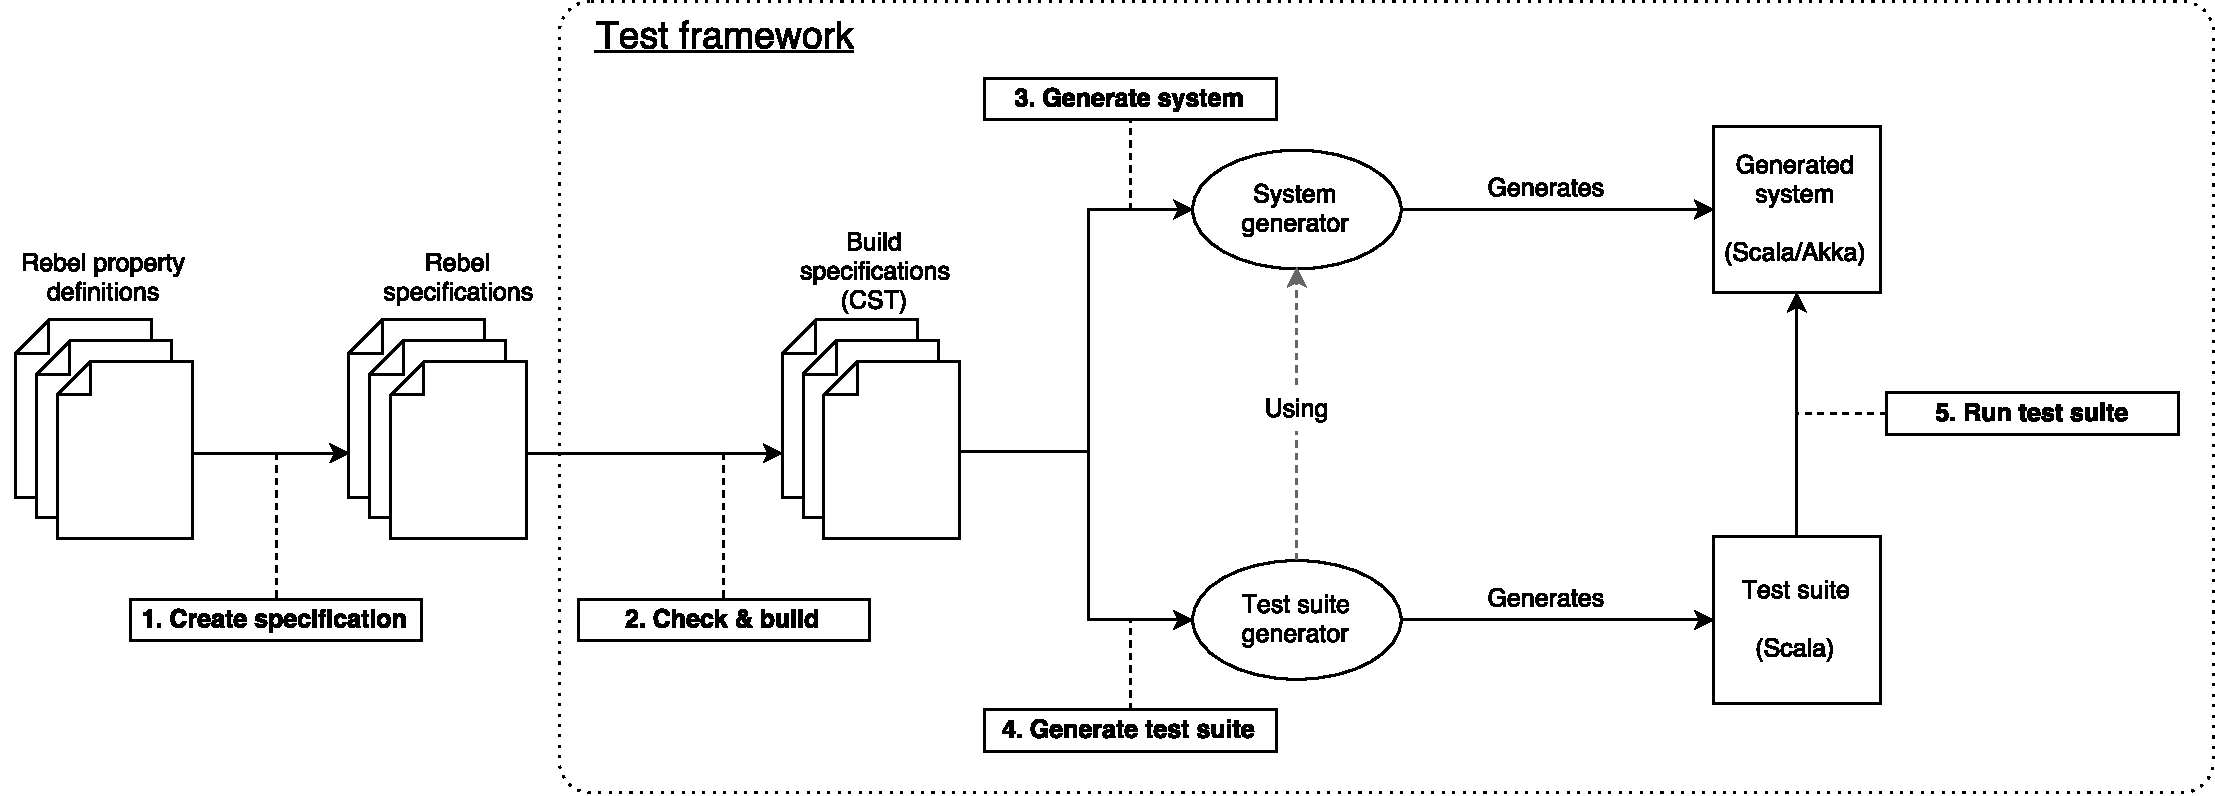
\includegraphics[width=\linewidth]{figures/testmechanics_overview}
%}
\caption{Overview of the test framework and the phases}
\label{fig:intro_tf_overview}
\centering
\end{figure}
\FloatBarrier\noindent
% End figure
%
% In short, describe steps:
% // (Steps also interesting for mechanics chapter)
% 1 Defining properties, define what is unknown yet and what it actually means.
% 2 Describe how tests can be generated out of this. From these properties to Scala tests. (Properties > Rebel events > Scala tests per event, with random values)
% 3 Describe how we measure our experiments
% 4 Evaluate the results. Can we reason about it? What have we covered and also what have we not covered?
%\pinfo{First defining properties, then small example}
We start off with defining the properties that are expected to hold on the
semantics of the generated code. With these properties, a \textit{Rebel}
specification can be created in which the properties are written down as
\textit{events} (\autoref{fig:intro_tf_overview}, phase 1). This phase is done
manually, the next phases are executed by the test framework.\\
\\
This \textit{Rebel} specification is checked by the type checker and then being
built, resulting in a CST (\autoref{fig:intro_tf_overview}, phase 2). The
\textit{Rebel} tool chain provides a generator to generate a Scala/Akka system
by using the CST of the specification (\autoref{fig:intro_tf_overview}, phase 3).
The same CST is used to generate the test suite
(\autoref{fig:intro_tf_overview}, phase 4). The test suite consists of multiple
tests based on the \textit{events} in the CST. Note that, as described earlier in phase 1,
the defined properties are written down as \textit{events} in the
\textit{Rebel} specification.\\
\\
As last, we run the test suite against the generated system (\autoref{fig:intro_tf_overview}, phase 5). After running the test suite, we analyse the results of the experiment. When one or more tests are failing, a bug is found. An
investigation of the failing case is needed to discover the actual bug is because the cause of the failing case is not clearly visible in the log.\\
\\
We evaluate the test framework in each experiment using test coverage and the number of bugs found as metrics. Based on the results of an experiment, we improve the test framework and continue to the next experiment. In the next experiment we run the test framework again with the improvements, analyse the results and evaluate the test framework again.

% Real short version
%Then we describe how these properties can be tested on the generator,
%using one property to demonstrate the working of the test framework. We can then
%run the tests suite against the generated system and check if this method
%actually works to detect bugs.\\
%\\
%\pinfo{Generate, run, evaluate results and improve again}
%Next, we generate tests for each of the defined properties and run these against
%the generated system. After running the test suite, the result is being
%evaluated. When one or more tests are failing, a bug is found. However, we need
%to investigate the failing case such that we discover what the actual bug is.
%After evaluating we improve our test framework and continue to run and evaluate
%the results again.

% % % % % % % % % % % % % % % % % % % % % % % % % % % % % % % % % % % % %
% Section: Contribution
\section{Contribution \& outline}
In \autoref{cpt:background} we describe the background (\textit{Rebel}, the
generator and property-based testing).
% - Definitions (properties)
% Before, in conclusion:
% We provided a definition of some types in \textit{Rebel} and described properties that should hold when using operations with these types. Since there were no clear definitions available yet of what these types exactly do, a contribution has been made to the \textit{Rebel} project, such that there are now some definitions and properties available. This also helps when reasoning about the implementation, as there is now a definition of what is expected. Although these definitions might change over time, it allows to reason back to an earlier starting point.\\
In \autoref{cpt:properties} we provide definitions of the properties that are
expected to hold when using the \textit{Rebel} language and its toolchain.
Allowing to reason about whether the properties are satisfied when using the
generator and answering the first research question:\rqOne There were
no existing property definitions of \textit{Rebel}, so we provide a starting
point for this with the focus on important properties of \textit{Rebel}.\\
\\
% - A way to automatically test the generator and generated system using Rebel, defining properties as events
% Before, in conclusion:
% We have shown a way to automatically test the generator using the \textit{Rebel} language and its toolchain, with the addition of our test framework. This is done by defining the properties that are expected to hold in the first case. Which can be translated to a \textit{Rebel} specification such that a system can be generated from it. Additionally using the generator when generating the test cases, so that the translation of expressions in the generator will be checked too. The different kind of properties should be able to detect unexpected behaviour.\\
The defined properties are being used to check the generator. In
\autoref{cpt:testmechanics} we describe this process in detail, which
contributes to answering the second research question:\rqTwo Throughout the experiments the test framework is improved too.\\
\\
% - Found number of bugs in generated system
% Before, in conclusion:
%A number of bugs have been found in the generated system, precision errors, overflow/underflow errors and even a compile error. These bugs are now known issues in this project, while these were unknown before. This shows us that this approach already worked in such a way that it is able to detect bugs in the generated system. It can be extended to detect even more bugs. With some modifications, it is also possible to use this approach with other generated systems, such that it can detect inequalities among these.\\
In the experiments (\autoref{cpt:experiment1}, \autoref{cpt:experiment2} and
\autoref{cpt:experiment3}), the test framework is run with the set of defined
properties. For each experiment we evaluate the results, investigate the failing
tests and evaluate the test framework. The results of the experiments contribute
to answering the third research question:\rqThree\\
\\
As last, we provide a discussion about the findings and answer the research
questions in \autoref{cpt:discussion}. Followed up by the conclusion in
\autoref{cpt:conclusion}.

% - Squants issues
% Before, in conclusion:
%In this approach, we identified two bugs, which were due to an open-source library used in the generated system, called \textit{Squants}. We reported these two issues, such that these can be fixed in a later version of the library.

% % % % % % % % % % % % % % % % % % % % % % % % % % % % % % % % % % % % %
% Section: Related work
\section{Related work}

% % % % % % % % % % % % % % % % % % % % % % % % % % % % % % % % % % % % %
% Subsection: Axiom-Based Testing
\subsection{Axiom-Based Testing}
In axiom-based testing (also known as property-based testing) axioms are defined which describe what the expected behaviour is of the system under test. It was introduced already in the early eighties, with \textit{DAISTS}~\cite{gannon1981data}. The axioms, which they write themselves, are being used as a basis for unit testing. The set of axioms describe the expected behaviour and are used to determine whether the implementation agrees with the defined axioms. Testing is automated, the user only defines the axioms and writes the implementation for this.\\
\\
\textit{DAISTS} focused on algebraic axioms, using the equality operator in the definitions. Axioms can also be specified in object-oriented style. An example of this is \textit{ASTOOT}~\cite{doong1994astoot} which applies the ideas of axiom-based testing. Axioms are defined in an object-oriented style, describing the methods used and the expected outcome. Whereas in algebraic style, the axioms are written more in a functional notation (as is done in \textit{DAISTS}). In this thesis, we use the algebraic style and use the equality as well as the inequality operators. Furthermore, we also have to define the expected behaviour of \textit{Rebel} expression.\\
\\
In~\cite{bagge2010axioms} axioms are used to automatically generate tests from these. They use the Concepts in C++ which contain the definitions of the axioms. Based on these Concepts they automatically generate tests for each defined axiom and run these tests to check whether the system under test satisfies these axioms. In this thesis, we define the properties (axioms) that are expected to hold in \textit{Rebel} and then generate tests based on these definitions by using the generator. The generated tests will then be run against the generated system that can be generated from a \textit{Rebel} specification. Our approach can be compared to the approach in~\cite{bagge2010axioms}, but we define the axioms in a \textit{Rebel} specification and then run the generated tests against the system that was generated based on the \textit{Rebel} specification that we created.

% % % % % % % % % % % % % % % % % % % % % % % % % % % % % % % % % % % % %
% Subsection: Random testing
\subsection{Random testing}
\pinfo{Describe random testing (FDRT)}
Random testing is a technique in which random values are being used as input
for the test cases. \textit{QuickCheck}~\cite{claessen2011quickcheck} and
\textit{Randoop}~\cite{pacheco2007randoop} are examples of random testing
techniques. These differ in how they automatically test systems and what
actually is being tested. \textit{QuickCheck} is based on property-based
testing, which we also use throughout this thesis. \textit{Randoop} on the other
hand is based on feedback-directed random testing.\\
\\
\pinfo{Describe FDRT}
With feedback-directed random testing, random tests are generated which will
immediately be run. The result of earlier test attempts can affect the next test
that is being generated, which can be seen as feedback for the next generated
test. This allows each test case to `learn' from earlier attempts and to create
unique tests.\\
\\
\pinfo{About Randoop, shortly how it works}
\textit{Randoop} is built for \textit{Java} projects and checks some built-in
specifications of \textit{Java} that can't be checked by the compiler. The test
cases are simple unit tests, consisting of a unique sequence of methods due to
the feedback of earlier attempts. The method sequences are unique because it
also checks whether the same case has already been checked. Since there can be
unlimited sequences of methods to test, the test suite will be terminated after
a defined timeout. Next, the result is determined and failing cases are being
reported, although when using this approach it cannot determine whether the
whole system is correct according to the \textit{Java} specifications. Instead,
it just wasn't able to find a case for which it fails. This is a useful approach
to generate unique tests, but its goal is to check systems built-in
\textit{Java} and thus is not compatible with the semantics of \textit{Rebel}.
It works with calling the \textit{Java} objects and using methods on those,
while the generated system consists of mainly states and events. When using an
approach like \textit{Randoop} with random input values, it cannot be known
whether the result of a specific transition was expected to succeed or fail.\\
% Can add DART here, if needed
\\
\pinfo{Our case, why existing approaches can't be used}
Approaches like \textit{QuickCheck}~\cite{claessen2011quickcheck} and
\textit{Randoop}~\cite{pacheco2007randoop} enforce the system under test to be
written in a specific language (\textit{Haskell} for \textit{QuickCheck},
\textit{Java} for \textit{Randoop}). For \textit{QuickCheck} there are
alternative solutions for other languages. In our case, we need to use
\textit{Rebel} when generating test cases, such that we test the generator when
generating the tests. Another reason why we can't use a method like
\textit{Randoop} is that \textit{Randoop} strictly checks for \textit{Java}
properties, which are not in line with the \textit{Rebel} language.

% % % % % % % % % % % % % % % % % % % % % % % % % % % % % % % % % % % % %
% Subsection: Testing generated systems
\subsection{Testing generated systems}
Using domain-specific languages leads to the creation of code generators to automatically generate executable code~\cite{boussaa2016automatic}. This is also the case for \textit{Rebel}, the toolchain provides some generators which use a \textit{Rebel} specification as input. These generators and the resulting generated systems can be automatically tested too. In~\cite{boussaa2016automatic} they focus on testing non-functional properties, namely testing the performance of the generated code. In~\cite{makki2016automated} the authors present a regression testing automation framework for a domain-specific language. They detect regressions in the generated systems by generating and executing test cases.\\
\\
In this thesis, we also focus on automatically testing the generator (by using the generated system) but we check more basic functionalities that are specific to \textit{Rebel} and its supported types.

% % % % % % % % % % % % % % % % % % % % % % % % % % % % % % % % % % % % %
% Subsection: Product-line testing
\subsection{Product-line testing}
In~\cite{al2016incling} the authors describe a way to efficiently test a software product line. A software product line consists of a set of software systems that share a common set of features. However, many different products can be created from such a software product line, adding a challenge to test each combination of those products. In~\cite{al2016incling} the authors introduce \textit{IncLing}, which efficiently tests combinations of these products and take already executed combinations into account when selecting a new combination. To determine the possible combinations they use the \textit{IPCL} algorithm introduced in~\cite{johansen2012algorithm}, an algorithm that can be applied to determine the combinations of software product lines at the size and complexity found in projects in the industry.\\
\\
\textit{IncLing} executes its tests sequentially by selecting a combination of features that were not covered in the previous test. This is a different way of testing each possible combination and ensuring unique test cases. In this thesis, we basically define the possible combinations by defining the properties (axioms) that we expect to hold in \textit{Rebel}. Additionally, the input values are determined random, allowing different combinations as in values. However, we do not test combinations of the properties combined, but test each individually. In our approach there could be some overlap over the various defined properties.
